\subsection{Các mô hình nhận diện địa điểm trực quan khác}
Các phương pháp nhận diện địa điểm trực quan thường được nghiên cứu theo xu hướng sử dụng ngữ cảnh của các ảnh trên đường phố. Việc có quyền truy xuất vào ảnh vệ tinh cũng như sự khuếch tán của rô-bốt trên không được trang bị camera đã mở ra một hướng phát triển mới. Một mặt, ảnh vệ tinh cho phép chúng ta có được đa dạng các góc nhìn cũng như một góc nhìn rộng hơn của khu vực. Mặt khác, chúng mở ra những thách thức như thiếu sót chi tiết trực quan.

\subsubsection{Định danh từ xa}
Trong truy xuất ảnh định danh từ xa, cũng như trong các tác vụ VPR cổ điển, mục đích vẫn là xác định vị trí ảnh nhận vào thông qua việc truy xuất ảnh tương đồng từ cơ sở dữ liệu. Do ảnh được chụp từ máy ảnh hướng xuống được trang bị trên một thiết bị bay hoặc từ vệ tinh dẫn đến việc ảnh sẽ phản ánh một khu vực địa lý lớn với nhiều vật thể có kích thước khác nhau. Các yếu tố vật thể dễ phân biệt ở tầng mặt đất như các tòa nhà lại không mang nhiều thông tin khi nhìn từ phía trên cao. Mặt khác, các yếu tố không mang quá nhiều thông tin hữu ích ở tầng mặt đất như đường xá lại quan trọng trong tác vụ định danh từ xa.

Dù cho có nhiều sự bất tương đồng, đã có những phương pháp VPR cổ điển được áp dụng để giải quyết bài toán định danh từ xa. Trong \cite{Tang2018UnsupervisedDF}, tác giả đề xuất sử dụng một phương pháp dựa trên túi-từ. Đầu tiên, các hình ảnh được chia thành các phân vùng sử dụng các phương pháp khác nhau. Sau đó, biểu diễn hình ảnh được xây dựng bằng cách kết hợp các đặc trưng ngầm được trích xuất bằng cách đưa mỗi phân vùng qua phần mã hóa của một mạng tích chập học sâu. Cuối cùng, túi-từ được tạo ra bằng cách sử dụng những biểu diễn này. Thay vì sử dụng phân vùng - tốn kém về mặt tài nguyên tính toán, \cite{Imbriaco_2019} đề xuất sử dụng kiến trúc DELF để trích xuất các đặc trưng cục bộ đáng chú ý sau đó kết hợp chúng thông qua trình tổng hợp VLAD. Ngoài ra, vì xác minh hình học khó áp dụng cho hình ảnh định dạng từ xa, các nhà nghiên cứu sử dụng mở rộng truy vấn dựa trên vector bộ nhớ \cite{7870636} để cải thiện kết quả truy vấn.

\begin{figure}[H]
    \centering
    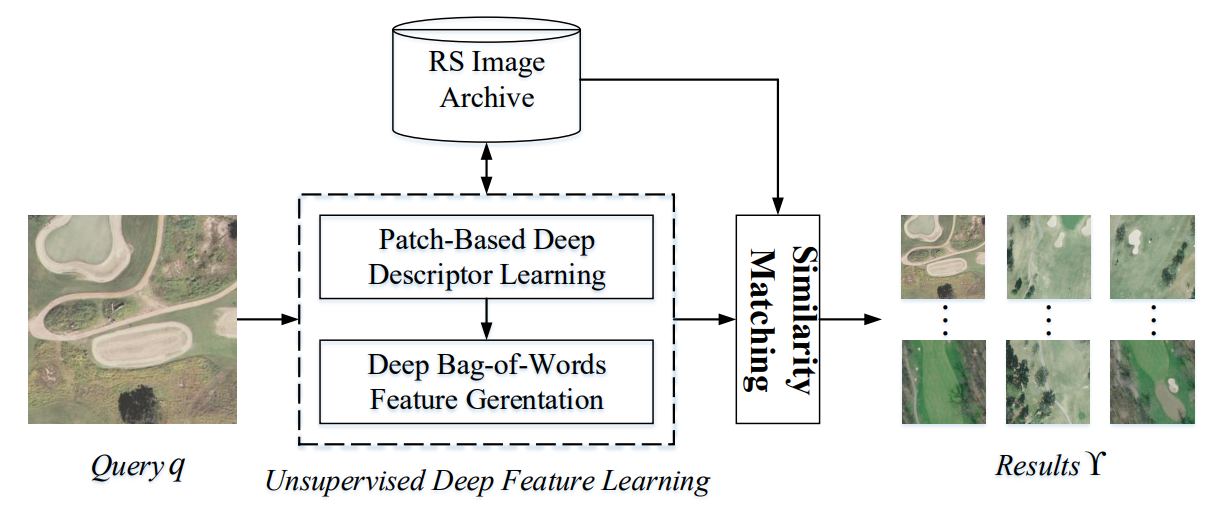
\includegraphics[width=0.6\textwidth]{pics/Chapter2/rsir.png}
    \caption{Minh họa mô hình DBOW \cite{Tang2018UnsupervisedDF}}
\end{figure}

\subsubsection{Truy xuất vị trí từ các góc nhìn chéo (cross-view geo-localization)}
Một công dụng khác của ảnh trên không được sử dụng trong nhận diện địa điểm trực quan là truy xuất vị trí từ các góc nhìn chéo. Cụ thể với hướng tiếp cận này, ảnh nhận vào sẽ ở mức độ mặt đất và ảnh từ cơ sở dữ liệu sẽ là ảnh trên không. \cite{Lin2015LearningDR} xem xét trường hợp cụ thể trong đó các hình ảnh trên không được lấy từ cơ sở dữ liệu Google Street View và được chụp với góc khoảng 45 độ cùng với bản đồ độ sâu thô. Thông tin này, cùng với giả định của mô hình máy ảnh trực giao, cho phép chiếu lại các hình ảnh tầng mặt đất lên tầng trên không và thiết lập các kết nối mặt đất-trên không. Những kết nối này sau đó được sử dụng như các mẩu dữ liệu để đào tạo một bộ trích xuất đặc trưng dựa trên CNN với mất mát đối lập. \cite{workman2015widearea} đề xuất huấn luyện một mô hình nơ-ron tích chập để trích xuất biểu diễn kết nối đầy đủ của các hình ảnh trên không bằng cách sử dụng một hàm mất mát $l_2$ để căn chỉnh những biểu diễn này với những biểu diễn được trích xuất từ mô hình đã được huấn luyện trước cho các hình ảnh mặt đất tương ứng. Góc nhìn chéo cũng được tận dụng trong \cite{Castaldo2015SemanticCM} cho trường hợp của hình ảnh hệ thống thông tin địa lý gắn với bản đồ ngữ nghĩa. Tương tự như \cite{Lin2015LearningDR}, một phép chiếu lại được sử dụng để chỉnh sửa hình ảnh tầng mặt đất, nhưng phép chiếu lại được áp dụng cho một bản sao có được phân chia ngữ nghĩa của ảnh truy vấn.

\begin{figure}[H]
    \centering
    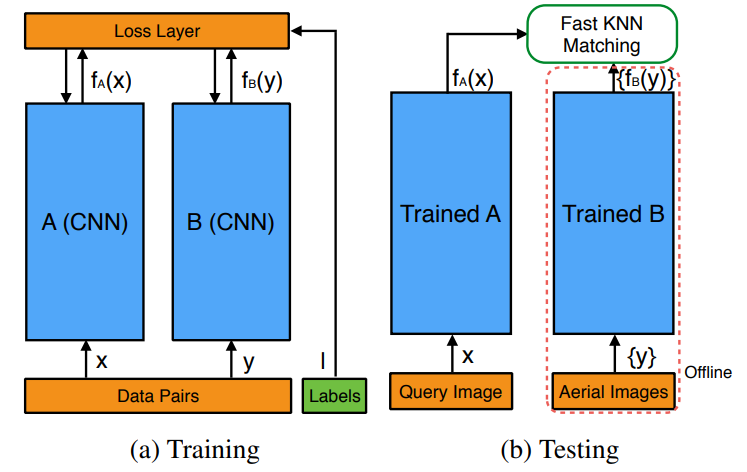
\includegraphics[width=\textwidth]{pics/Chapter2/wherecnn.png}
    \caption{Minh họa mô hình DBOW \cite{Lin2015LearningDR}}
\end{figure}